\documentclass{IEEEtran}
\usepackage{graphicx}
\usepackage{verbatim}
\usepackage{url}
\usepackage{color}
\usepackage{array}
\usepackage{multirow}
%\usepackage{subfigure}

%%%%%%%%%% verbatim related
\usepackage{fancyvrb}
\usepackage{fixltx2e}
\fvset{framesep=2mm,fontsize=\scriptsize,framerule=.1mm,numbersep=1mm,commandchars=\\\{\}}
\usepackage{listings}
\usepackage[usenames,dvipsnames]{xcolor}


%%%%%%%%%%%%%%%%%%

\newcommand{\eat}[1]{}
\newcommand{\rmv}[1]{ #1}
\newcommand{\sysname}{XXXXXX}

\newif\ifrev
% comment out the following line after the revision is done
\revtrue
\ifrev
  \newcommand{\cappos}[1]{{\color{red} [Justin: #1]}}
  \newcommand{\reznik}[1]{{\color{blue} [Leon: #1]}}
  \newcommand{\weiss}[1]{{\color{green} [Richard: #1]}}
 \newcommand{\yanyan}[1]{{\color{blue} [Yanyan: #1]}}
\else
  \newcommand{\cappos}[1]{}
  \newcommand{\reznik}[1]{}
  \newcommand{\weiss}[1]{}
\fi

\begin{document}

\title{A Trust Evaluation Framework for Mobile Devices and Applications}
\author{Bart}

\maketitle


\begin{abstract}
Evaluating trust
 is a challenge for many computer systems.  Smartphones and mobile devices install software from a 
wide range of sources.  As these devices become
more popular, the risks of associated malware will become more significant.
One of the features of these platforms is that they are rich in
sensors\footnote{In this work, smartphone sensors are broadly defined as hardware components that can record phenomena about the physical world.}.  These sensors can be a risk to privacy in that they could leak information about the 
user and user activities.  On the other side, they can also be used as an
advantage if they can be used to evaluate trust.
%leak information about any malware that is running on it.  

This paper builds  a hierarchical security evaluation 
\yanyan{eval security or trust?} framework 
that uses sensors to evaluate trust and detect anomalies. We examine the results 
of two empirical studies where this framework is applied.  
The first study involves monitoring resource utilization.  For example, malicious code 
injected into an app or OS utility could manifest as an increased consumption in 
system resources, such as CPU or network communication. Sensor values like battery level 
and CPU utilization can detect this.  The second study involves erroneous sensor values. 
For example, malwares that could produce an intentional or inadvertant effect on sensors, such 
as accelerometers and GPS receivers, could be detected by measuring anomalies 
in these sensor values. Our approach is two-fold: evaluating trust based on metrics 
and models, \yanyan{more specific what the metrics and models are?} and 
using this evaluation to detect anomalies as a way to improve security in general.


\eat{For many people, smartphones and other mobile devices serve as a technical interface to the modern world.
These smart devices have embedded on-board sensors, such as accelerometers, gyroscopes, GPS sensors, and
cameras, which are very useful.

This work describes \sysname, a hierarchical framework for checking consistency of sensors 
from multiple devices.  In addition, it relies on Blursense, a dynamic, fine-grained, flexible access
control mechanism, acting as a line of defense that allows users to define and addprivacy filters. 
As a result, the user can expose filtered sensor data to untrusted apps, and researchers can collect 
data in a way that safeguards users' privacy.}  %end comment
\end{abstract}

%\IEEEpeerreviewmaketitle

\section{Introduction}

Android and mobile devices and smartphones are becoming increasingly popular.  The number of mobile phones
sold has surpassed the number of laptops, and in 2014 it was XXX. Google is reported to have more than
a billion active users of Android-based devices.  As their popularity increases, so does their value as
a target for malware.  There are many possible risks.
Many people use smartphones for financial transactions.  Attackers could get personal
information for systems administrators and CIOs from their phones and use that for spear phishing.  
%mention security and privacy issues 

The more sophisticated mobile devices become, the more complex the threat model is, and the more opportunities
for vulnerabilities.  Finding viruses and other malware using software signatures is less and less likely to
work.  What is needed is a system-wide  aproach that involves assessing trust for the different
components by detecting anomalies in sensor behavior and history of the component.  
In recent research done by Hoffman, et al.~\cite{hoffman}, the authors developed a hierarchical 
mechanism that is scalable and expandable for evaluating security of
Android smartphones by investigating various sources of information regarding 
the mobile devices. 
%
The three sources of information that they integrate are:
analysis of installed applications using metadata provided by the Google Play store,
usage information coming from security tools embedded in the OS, and 
validation of the device by inspection of sensor data.  
The sensors in this context refer to any function that
measures the physical state of the smartphone.  This can include geolocation, accelerometers, CPU 
utilization, and battery charge.

In this paper we focus on the second and third sources: inspection and comparison of sensor values.
\yanyan{need more text..}

The contributions of this paper include. \yanyan{complete..} % this will describe the problem and applications, threat models
\section{FRAMEWORK UMBRELLA ARCHITECTURE AND DESIGN}
%This is a summary of section 2 in the Hoffman paper

A hierarchical trust analysis can look at the entire system and combine measurements from multiple sources, making
it more powerful than measuring a single component or layer.
In this section we discuss a comprehensive mechanism that provides a scalable and extendable methodology of security evaluation and analysis for Android based mobile devices. 

Quality and security evaluation is a complex subject, which depends on multiple characteristics, e.g. sensor accuracy, the rate of encrypted messages, and/or the probability of a system's breakdown over a given period of time. Its evaluation should integrate various metrics ranging from the accuracy and reliability of the data sources to the security of the procedures and tools used. The major research challenge of the framework design is integrating the numerous metrics needed to characterize a device and its security while working with limited resources and processing power. We address this challenge by hierarchically structuring the security metrics composition as well as by designing a specialized calculus to evaluate the overall security. 

Therefore, the major innovative emphasis in our framework design is put on the integration of a wide variety of indicators and their evaluation procedures. The framework procedures output the overall data quality evaluation indicators and additionally calculate the individual product of metrics characterizing system features which are then used to produce recommendations for improvement. The application will facilitate decision making, improve performance and increase accountability through the collection, analysis, and reporting of relevant performance-related data. This design facilitates the framework extension and makes it accessible for other metrics inclusion as well as an easy modification and improvement.
Current implementation of this framework provides the following metric functionality: 
\yanyan{according to intro, we only look at 2 and 3. Better merge this sec with intro.}

\begin{enumerate}
\item Analysis of the installed applications through the application specific metadata provided by the Play store. Applications represent the largest security and privacy risk to a device and user's data. The data provided by the Play store leverages the experiences of millions of users and holds all data associated with the distribution of an application including its associated documentation. The Play store also provides meta-information about applications which provides useful characteristic data about an application. This data can be used to assess an individual applications risk. Rules were generated to classify each application into a risk impact class based on this meta-data. The combined security classes of all applications installed on a device would be used to create a security risk rating for the whole device.

\item The usage verification of security tools embedded into the operating system and proper preventative security practices. Android provides users with many different tools which increase the security and privacy of their devices in addition to updates to patch exposed vulnerabilities. When properly used, these tools improve the security of the devices. In order to gather a comprehensive overview of the software running on a mobile device an analysis of the operating system and user settings is performed. First the operating system is checked to confirm that it is running the most recent version available. Second the personal security settings on the device are examined to determine if the user is utilizing the appropriate tools to secure the device. These operating system verification checks combined generate a score, which is used in the security and privacy framework operation result.

\item Validation of the device evaluation through inspection of the sensor data. Detection of the compromised devices can sometimes be determined by the analysis of the spurious output of its internal sensors. Verifying the validity of the sensors can detect security and quality problems of the device that would be missed by the other subsections. Most mobile devices now come equipped with a variety of sophisticated sensors which are capable of very accurate measurements of their surrounding environment. As the data from these sensors are used in more security critical applications the importance that these data remain accurate and legitimate should not be underestimated. For example, data from the GPS sensor can be verified to be trustworthy and assigned a security rating. The combination of ratings from all sensors would produce the devices sensor security risk score.
\end{enumerate}


Unlike other reported tools available, our framework has an umbrella structure that allows for an integration of various diverse security evaluation mechanisms and results. This open architecture provides an opportunity for an easy and simple extension and inclusion of various tools as well as a combination or diverse target areas. At the same time, the self-learning ability allows for its optimization towards a particular device and a criteria set. Each of these procedures given above generates a security risk rating, which is then integrated together as part of the umbrella framework. This framework takes into account the varied landscape of mobile devices and is designed to be flexible and easily adaptable to the changing security environment. Based on this design and contribution of each of the procedures could be adjusted depending on the target.
\yanyan{I don't think we do self-learning or risk rating. Delete? Otherwise IMHO would be considered 
as over claim by reviewers.} % summary of section 2 of the Hoffman paper
\section{Measuring app behavior}

Anomalous behavior of a smartphone may be due to malicious adulteration of an application or
the operating system, or installed during the hardware manufacturing chain.
In order to be able to detect this
behavior, we first need to establish baseline measurements for 
normal behavior. We focus on metrics that are observable 
without requiring inspection of the app's source or binary code
because obfuscation techniques are very sophisticated and will continue to be developed.
We have enhanced existing debugging with additional internal sensor measurements to inspect app behavior.
Aggregate metrics, such as battery voltage and CPU usage are easy to collect.  However,
they can also be influenced by random and extraneous factors.

\subsection{Battery voltage}
A proxy metric for the amount of remaining 
energy in the battery. Any kind of activity on the device will result 
in a change of battery voltage, but the resolution of readings (both 
in time and in voltage) only allows for coarse, averaged measurements 
under general, non-lab conditions.

If the circumstances can be controlled tightly, then approaches like 
\textit{Eprof} \cite{pathak2012fine} can be used to estimate energy consumption 
of individual activities and assign credit to likely originators.


\begin{table}[ht]
\centering 
\scriptsize
\begin{tabular}{|l||l|l|l|}
    \hline
    {\bf Time} & {\bf 15s} & {\bf 60s} & {\bf 10min} \\
    \hline
    \% of total battery use with ads (avg)  & 81.4\%   & 53.0\%   & \\
    \hline
    \% of total battery use with ads (max) & 86.0\%  & 61.5\%  & 11.9\%  \\
    \hline

\end{tabular}
\caption{A comparison of battery use with anomalous adware compared with normal.
The ad was 15 seconds.}
\end{table}

\subsection{CPU usage}

\begin{figure*}[ht]
\centering
\includegraphics[width=6in]{no_AdsDisplay_10s.png}
\caption{A typical session in Traceview, the execution log viewer.
WebViewCoreThread is busy, but main thread's workload is very light.  main is reponsible for 
the user interface, in general.  WebView is reponsible for rendering ads using the webkit library}
\label{fig:cpu-no-ad}
\end{figure*}

\begin{figure*}[ht]
\centering
\includegraphics[width=6in]{traceview.png}
\caption{A session in Traceview, with anomalous Ads.  Notice that main is doing much more work and
there are other threads that are getting significant CPU time.}
\label{fig:cpu-ad}
\end{figure*}

Similar to battery voltage, monitoring the overall CPU usage 
(which is an operation requiring no special privileges on Android) 
can be used to get a coarse-grained overview of consumption. 
However, the existing debugging and tracing interfaces permit 
finer-grained views as well. Assuming an app is not designed to 
evade or complicate debugging deliberately, the 
\textit{Dalvik Debug Monitoring Service} (DDMS) 
% https://developer.android.com/tools/debugging/ddms.html
provides syscall-level insight.

Figure~\ref{fig:cpu} shows a typical  
session in Traceview, the execution log viewer.
\yanyan{did you mean Figure~\ref{fig:cpu-no-ad}? how about 
Figure~\ref{fig:cpu-ad}? We should mention both.}
% Current figure (MD5 46fbce842e071dfb8f321c9645c6b411) courtesy of Tao Li.
The app under scrutiny comprises several threads with different 
temporal activity patterns. Some threads bear names indicative 
of their performed functions. Colored bars in the threads' activity 
timelines further detail call-level interactions with app and system 
libraries, with the height of sub-bars proportional to the frequency 
of specific calls.

Other log views (not shown) list all of an app's threads, show the 
call stack for each, and display cumulated and individual CPU time 
consumption, and relative usage.


%%% http://www.sigmobile.org/mobisys/2012/program.php#ses5

\subsection{Network usage}

Android provides a number of built-in features allowing the observation 
of a device's network conditions for any app granted the 
\texttt{ACCESS\_NETWORK\_STATE} permission. 
The \texttt{ConnectivityManager} class lets an app discover the 
current connectivity status and type (WiFi, 3G, Bluetooth, Ethernet). 
For cellular access such as LTE or 3G, the \texttt{TelephonyManager} 
class makes available further detail. The stateful nature of cellular 
data connectivity is reflected by various indicators of data activity, 
thereby allowing any app to detect when other apps transfer data over 
the cellular interface.  The Application Resource Optimizer project
(ARO\footnote{See \url{https://github.com/attdevsupport/ARO}}) and \cite{Ricciato2010551} 
provide further insights into what is 
essentially radio resource control (RRC-based type of diagnostics).

%%% https://developer.android.com/reference/android/telephony/TelephonyManager.html (See NETWORK_TYPE_* and DATA_* states)
%%% https://developer.android.com/reference/android/net/ConnectivityManager.html (See TYPE_*)
%%% https://developer.android.com/reference/android/net/NetworkInfo.html#isConnected%28%29

If the device is \textit{rooted} (i.e., system-level administrator 
privileges are available to the user launching an app), standard 
packet tracing tools such as \texttt{tcpdump} can be used to 
record the exact data transferred across network interfaces. 
However, the precondition is not met on almost any commercial stock 
firmware.
% Note: tcpdump doesn't allow inspection of encrypted content either. 
% There are approaches adding a system-level certificate to MITM on 
% HTTPS connections see for instance https://github.com/egirault/googleplay-api ,
% but I think this also requires root.

When packet-level tracing on the device is infeasible, the network 
connection of the device might be tapped instead. A natural place 
for this would be a WiFi router acting as the device's gateway. 
Neither on-device nor on-path packet tracing allow decryption of 
HTTPS and other encrypted network traffic. However, at least for 
HTTPS implementations using the system libraries, deliberate 
man-in-the-middle (MITM) attacks on traffic may be performed 
by adding a self-provided certificate to the system's certificate 
storage, and redirecting outgoing HTTPS traffic to a local proxy 
server using that certificate.
  % what is anomalous behavior, how are resources monitored?
\section{Trust Evaluation Testing and Verification}
\label{sec:geolocation}
%Description of the OBD system, how data can be retrieved from the car.
Another form of trust evaluation is verification based on the use of sensors on multiple devices~\cite{ju2012neteye}.  For example,
a smartphone may communicate directly with a smartwatch or on-board diagnostics (OBD)
sensor on an automobile.  These other devices have sensors with the same
functionality as some of the sensors on the smartphone.  If there is a discrepancy in the sensor measurements, 
the trust evaluation of the device can be reduced unless it can be determined that the trust metric for the 
external sensor data is low.
% describe what data is collected, how it is stored, and how it might be used.
% we can include a graph of spped error vs time and the picture of the car route
We introduce a case where smartphones communicate with an in-vehicle OBD sensor
to get geolocation information, such as speed, engine RPM, fuel consumption, 
etc.

\subsection{Vehicle data collection}

Vehicular data collection consists of a process on a mobile 
device that directly communicates with in-vehicle sensors and collects sensor 
data~\cite{sensor}. Data can be encrypted and transferred to a
centralized server for permanent data storage. 
To deploy such a process on a mobile device, a device owner first installs an
app~\cite{sensor-app} on their device\footnote{Currently, Android smartphones 
and tablets are supported.}. Since we are interested in
vehicular data, the target group of device owners are also the vehicle 
owners. An owner simply inserts a WiFi 
OBD~\cite{obd} sensor into the car's OBD port (located under the steering wheel),  
%\linda{I don't think they insert their sensor into the car. Do they insert it into something specific in the car (e.g., a usb port)? That would make sense. Anyway, I think you need to be more specific in stating what gets connected to what} 
and connect a 
smartphone or tablet to the sensor, which also runs as a WiFi access 
point. Note that OBD systems are available in most cars and light trucks 
on the road today~\cite{obdconnector}. 
\eat{Therefore, our 
infrastructure does not require extra installation of specialized  
hardware or equipment~\cite{reininger2015first}. } % end comment
Trust evaluation could be used to determine if the phone should trust the car,
or vice versa, as well as whether the user should trust the combined system.

The vehicular data is uploaded to a remote server by the app
which runs in the background of the mobile device and communicates
with an in-vehicle OBD sensor. The device owner need not worry about having to
interact with the app or about being interrupted while using the smartphone. 
Note that all code runs in a secure sandbox in our 
app~\cite{sensor-app}, which limits the amount of storage, network, 
memory, battery, and CPU resources used by that code~\cite{Cappos_CCS_10}. 
To protect the end user's device from malicious attackers, the sandboxed 
code is securely isolated from other programs on the same device.
Any bugs in the code will be contained in the sandbox, and will not 
affect the rest of the user device~\cite{Cappos_CCS_10}. 
%Once our prototype data collection application is installed and running on an Android smartphone with Sensibility, the end user need not worry about interacting with a user interface on the Android. Rather, once the user inserts their WiFi OBD sensor into the car and connects their Android smartphone to the sensor running as a wifi access point, our 
%

At the remote server, the vehicular sensor data collected from 
multiple end user devices is stored in a non-relational database. 
The collected data is stored in JSON format.
The collected data set can be visualized on Google Maps to 
identify fuel efficient routes, routes with higher traffic activity.
Furthermore, the data set could also be used to detect reckless or illegal driving behaviors,
in which case trust metrics would be significant.

\eat{
\begin{figure}
\scriptsize 
\begin{Verbatim}
\{
  \textbf{"sensors"}: \{
    \textbf{"speed_car"}: \textcolor{red}{60},
    \textbf{"maf_car"}: \textcolor{red}{4},
    \textbf{"rpm_car"}: \textcolor{red}{114},
    \textbf{"gps_phone"}: \{
      \textbf{"error"}: \textcolor{red}{null},
      \textbf{"id"}: \textcolor{red}{0},
      \textbf{"result"}: \{
        \textbf{"network"}: \{
          \textbf{"time"}: \textcolor{red}{1407200660927},
          \textbf{"speed"}: \textcolor{red}{60},    
          \textbf{"altitude"}: \textcolor{red}{4.099999904632568},
          \textbf{"bearing"}: \textcolor{red}{82.6999694824219},
          \textbf{"provider"}: \textcolor{OliveGreen}{"gps"},
          \textbf{"longitude"}: \textcolor{red}{-73.986706},
          \textbf{"latitude"}:\textcolor{red}{40.694010},
          \textbf{"accuracy"}: \textcolor{red}{7},
        \}
      \}
    \},
    \textbf{"id"}: \textcolor{OliveGreen}{"310410696731709"},
    \textbf{"time"}: \textcolor{SkyBlue}{"ISODate"}(\textcolor{OliveGreen}{"2014-08-05T21:04:07.183-04:00"})
\}
\end{Verbatim}
\caption{JSON document of vehicular data.}
\label{fig:json}
\end{figure}
}  % end comment


\eat{
\subsection{Data store}
Given the variety of sensors on a smartphone,
sensor measurements come in different forms. 
As shown in Figure~\ref{fig:json}, many types of sensor data have complex structure.
As a result, we decided to use a non-relational database, 
MongoDB~\cite{mongodb}, for storing sensor data. MongoDB has a Binary 
JSON (BSON) document-style structure identical to that shown previously 
in Figure~\ref{fig:json}, albeit converted into binary as its name suggests. 
This provides the scalability that is crucial to our system and that allows dynamic storage of 
new sensors, as needed. } % end comment

\subsection{Geolocation data analysis}

\begin{table}
\scriptsize
\centering
\caption{\small Speed comparison: GPS speed comparing to OBD speed.}
\label{tab:speed-diff}
\begin{tabular}{|p{.06\columnwidth}|p{.18\columnwidth}|p{.22\columnwidth}|p{.28\columnwidth}|}
\cline{2-4}

%\multirow{3}{*}{Statistics}

\multicolumn{1}{c|}{}  & \textbf{GPS speed} & \textbf{Vehicle speed} & \textbf{Speed difference}  \\ \hline

% Mean & 5.559 & 1.568 & 0.003606 \\ \hline 

Med & 53.0~kph & 54.9~kph & 2.15~kph \\ \hline

STD & 12.79~kph & 13.61~kph & 4.57~kph  \\ \hline

\end{tabular}
\end{table}

\begin{figure}
\centering
\includegraphics[width=4in]{speed.png}
\caption{Speed difference and accuracy.}
\label{fig:speed-diff}
\end{figure}

Using the aforementioned measurement, we collected speed data from both GPS 
on the smartphone inside a vehicle, and the speed via the OBD sensor. 
The data from these two sources can corroborate to verify normal or abnormal 
geolocation data. Table~\ref{tab:speed-diff} shows the median and standard deviation
of the speed measured by GPS and OBD sensor, over 58 data samples collected. 
The overall statistics do not show any anomaly in speed. However, when plotting 
individual data samples, we can see a data outlier in Figure~\ref{fig:speed-diff}. 
Excluding this point, the rest of the data samples roughly follow a Gaussian 
distribution. This outlier seems to be due to the initialization of the
GPS sensor.  Initially, the GPS parameters are underconstrained, leading to a large 
geolocation error that is then rapidly reduced as more measurements are made.


\begin{figure}
\centering
\includegraphics[width=4in]{car.png}
\caption{The difference between the OBD sensor speed and GPS speed decreases slightly as vehicle speed increases.}
\label{fig:car}
\end{figure}

To further investigate the speed data, we plot the differences between 
vehicle speed and GPS speed, and compare the differences against 
the varying vehicle speed. As shown in Figure~\ref{fig:car}, the speed 
differences vary linearly with the vehicle speed 
(other than the outlier), i.e., the 
higher the vehicle speed, the smaller difference between vehicle 
speed and GPS speed. 
A minimum mean square error (MMSE) linear fit is shown in the figure.

\begin{figure}
\centering
\includegraphics[width=4in]{time.png}
\caption{After the initialization of the GPS sensor, the difference between the  OBD sensor speed and GPS speed remains between 0 and 12~kph.}
\label{fig:time}
\end{figure}

We also investigate the vehicle and GPS speed differences over time, as shown
in Figure~\ref{fig:time}. From the figure, we can conclude that excluding the outlier, 
the differences between 
vehicle speed and GPS speed fluctuate around a constant value over 
time. 

\eat{
\eat{
1) Overview of the Solution: Today's smartphone OS typ-
ically exposes resources based on a static policy. Such per-
missions are often much more than necessary. Several related
work has been proposed to refine or reduce permissions on
mobile platforms [18], [29], [17], [30] via modifying the
device platform. BlurSense allows untrusted parties to add
privacy filters from user space. Multiple security vendors
can efficiently and effectively collaborate to strengthen user
privacy.} %end comment

BlurSense provides a way to control the precision and accuracy of the GPS
sensor.  We show how blurring the GPS location affects the difference between
speed measured by a car speedometer and communicated via the OBD port to
a smartphone, similar to our experiment in section~\ref{sec:geolocation}.

\begin{figure}
\centering
%\includegraphics[width=3.5in]{}
\caption{Speed difference vs time with blurring of the GPS data.}
\label{fig:blur-GPS}
\end{figure}


\eat{
 BlurSense
provides a programmable privacy protection framework. Users
not only gain full transparency of what information is captured
on their devices, but also have full control over how much
information they would share with the rest of the world -
a secure personal data ecosystem. After installing BlurSense,
a user can install software from a third party (like a security vendor) that performs custom sensor filtering actions in
response to application requests. For example, an application
could be prevented from using motion sensors when running
in the background, or precise GPS data could be abstracted
to a neighborhood or zip code. 
BlurSense
provides effective controls for smartphones, much like Flash and JavaScript
filtering tools protect laptops and desktops (e.g., NoScript~\cite{noscript},
AdBlock~\cite{adblock}, FlashBlock~\cite{Flashblock}). 

2) What BlurSense Provides: Seattle provides a sensor
interposition mechanism and a sandboxing mechanism that
make it easy to implement privacy filters. A user can let a third
party have access to their sensor data from within a security
and performance isolated container [20]. By leveraging this
security, the user provides minimal trust in the third party,
but allows them an easy way to code their filters. This
functionality also automatically handles multiple privacy filters
from different parties through the sandbox policy composition
functionality~\cite{Cappos_CCS_10}.
Researchers who use BlurSense will build a mechanism
to trap the requests from generic  applications and pass them
into BlurSense (a proof-of-concept for Android has already
been built). They will build and manage an ``App Store'' for
BlurSense to allow users to locate privacy filters they wish
to apply. These may range from sharing sensor data with
researchers by reducing the precision of sensor values, salting
and hashing sensor values for anonymizing collected data,
or completely denying access to individual (or all) sensors.
For a particular sensor, a filter might perform an action such
as blurring the resolution of photos and video taken by the
camera, removing access point information from WiFi scans,
or omitting the motion sensor data completely. Security and
privacy groups can easily build and disseminate their own
privacy filters they recommend to users by adding them to
BlurSense app store. Therefore, BlurSense is able to handle
the three categories of threats in Section


\eat{To protect smartphone users'
privacy, Blursense provides a dynamic, fine-
grained, flexible access control mechanism, which incorporates
privacy filters in user space [19], [20]. } % end comment

We want to let users
choose defenses freely in a marketplace so that different
vendors can build them.
Specifically, it implements a framework of reference
monitors, to enforce mandatory access control to sensor data
in real time. A reference monitor is a method or function that
implements an access control policy for a set of resources and
is usually specified in terms of what capabilities are allowed.
The access control that we are concerned with in this paper is
for sensor data with respect to applications in user space. If
such an application needs to access any of the sensor data, the
second line of defensive (reference monitors) will come into
play, mediating every access to sensor data. 
%As a result, a user should be able to combine solutions from different vendors.
If a vendor's product is vulnerable to attack or the vendor is malicious,
the user can still be protected.
According to the semantics of the access requests and the
current context, when a remote procedure call is made to the
Android OS to request sensor data, it will be handled by a
reference monitor. Based on a sensitivity of the application,
the data returned may be filtered, dropped or passed through.
Note that the reference monitor cannot pass on data that is
blocked by the manifest file because it is layered on top of
whatever privacy and security mechanisms that are in place at
the OS level. If the request is for highly sensitive sensor data,
then the request might be simply rejected. Otherwise, if the
request is for medium-level sensitive sensor data, the request
might get through, but the returned data has reduced resolution.
If the request is for low-sensitive sensor data, then the return
results need to be processed, e.g., by filtering or obfuscation.
BlurSense can be used with Sensibility Testbed~\cite{cappos-sensibility}, 
which provides
a rich and extensible collection of sensor data from Android
devices 
}
} % end comment
 % summary of sensibility platform with some blursense added and
            %  description of the OBD system
\section{TRUST EVALUATION METRICS BASED ON THE SUPPORTED PRIVACY LEVEL}
\label{sec:blursense}
Privacy is part of trust evaluation.
The greater the level of privacy that an application or device can provide, the greater its trust evaluation would be.
A privacy enhancing system such as BlurSense~\cite{cappos2014blursense} can improve the trustworthiness of an Android device  
 by filtering or restricting the sensor data that an application can access.
In addition,
one can apply trust metrics to automate the application of Blursense itself.  For example, if an app has a low trust evaluation,
then BlurSense can restrict the sensor data that the app has access to.

\subsection{The Trust Evaluation Model}
Although the sensing capabilities enhance the convenience of user interfaces and
application usefulness, they also raise serious privacy
concerns~\cite{shabtai2010google}. For instance, through accessing sensor data,
malicious applications could retrieve sensitive information about the mobile
phone users, such as location, passwords, and credit card numbers~\cite{xu2012taplogger, 
miluzzo2012tapprints, xu2009stealthy, cai2011touchlogger}. They
even might be able to send these sensitive information to remote
attackers~\cite{schlegel2011soundcomber, marquardt2011sp}. There
has been alarming news about privacy breaches of personal data on smart devices:
26\% of Android apps in Google Play can access user's personal
data~\cite{toomuch}; an iOS app auto-posts false piracy accusations on users'
Twitter accounts~\cite{tweetios}; apps can steal sensitive information like
passwords using the smartphone's motion sensors to determine tapped
keys~\cite{xu2012taplogger}; and a huge botnet that is collecting sensor data
was discovered on more than a million end user smartphones~\cite{botnet}. The
Federal Trade Commission (FTC) even recommended that mobile platforms should
provide in-time disclosures to users of accessing sensitive content on smart
devices~\cite{ftc}. 

\subsection{Applying Trust Metrics to BlurSense}
Trust metrics can also be used by privacy enhancing tools such as BlurSense to limit access to sensor data.
The current access control to the smartphone resources,
such as sensor data, is static and coarse-grained. 
%However, such defense is pre-determined by the manufacturer. 
Take the
Android platform as an example, the access permissions are
either granted or denied completely during the installation of
applications based on a request XML manifest file. As a result,
applications may ask for more permissions than are actually
required for operation. Having been granted the requested
permissions, applications have access to those resources permanently. 
A trust metric could be used during installation of an app to decide whether or not
to deny access specified in its manifest file.  
A better approach is to restrict access to sensor data in a
dynamic and fine-grained framework.
Some systems that have been proposed to address this
issue require modifications to the Android
platform~\cite{conti2011crepe, hornyack2011these}. This increases the cost of maintenance, is
less flexible and cannot be used in legacy systems. In addition,
the user would need to trust that the new operating system is
not malicious and is not more vulnerable than the standard one.

\begin{figure}%[htd]
  \centering
  % Requires \usepackage{graphicx}
  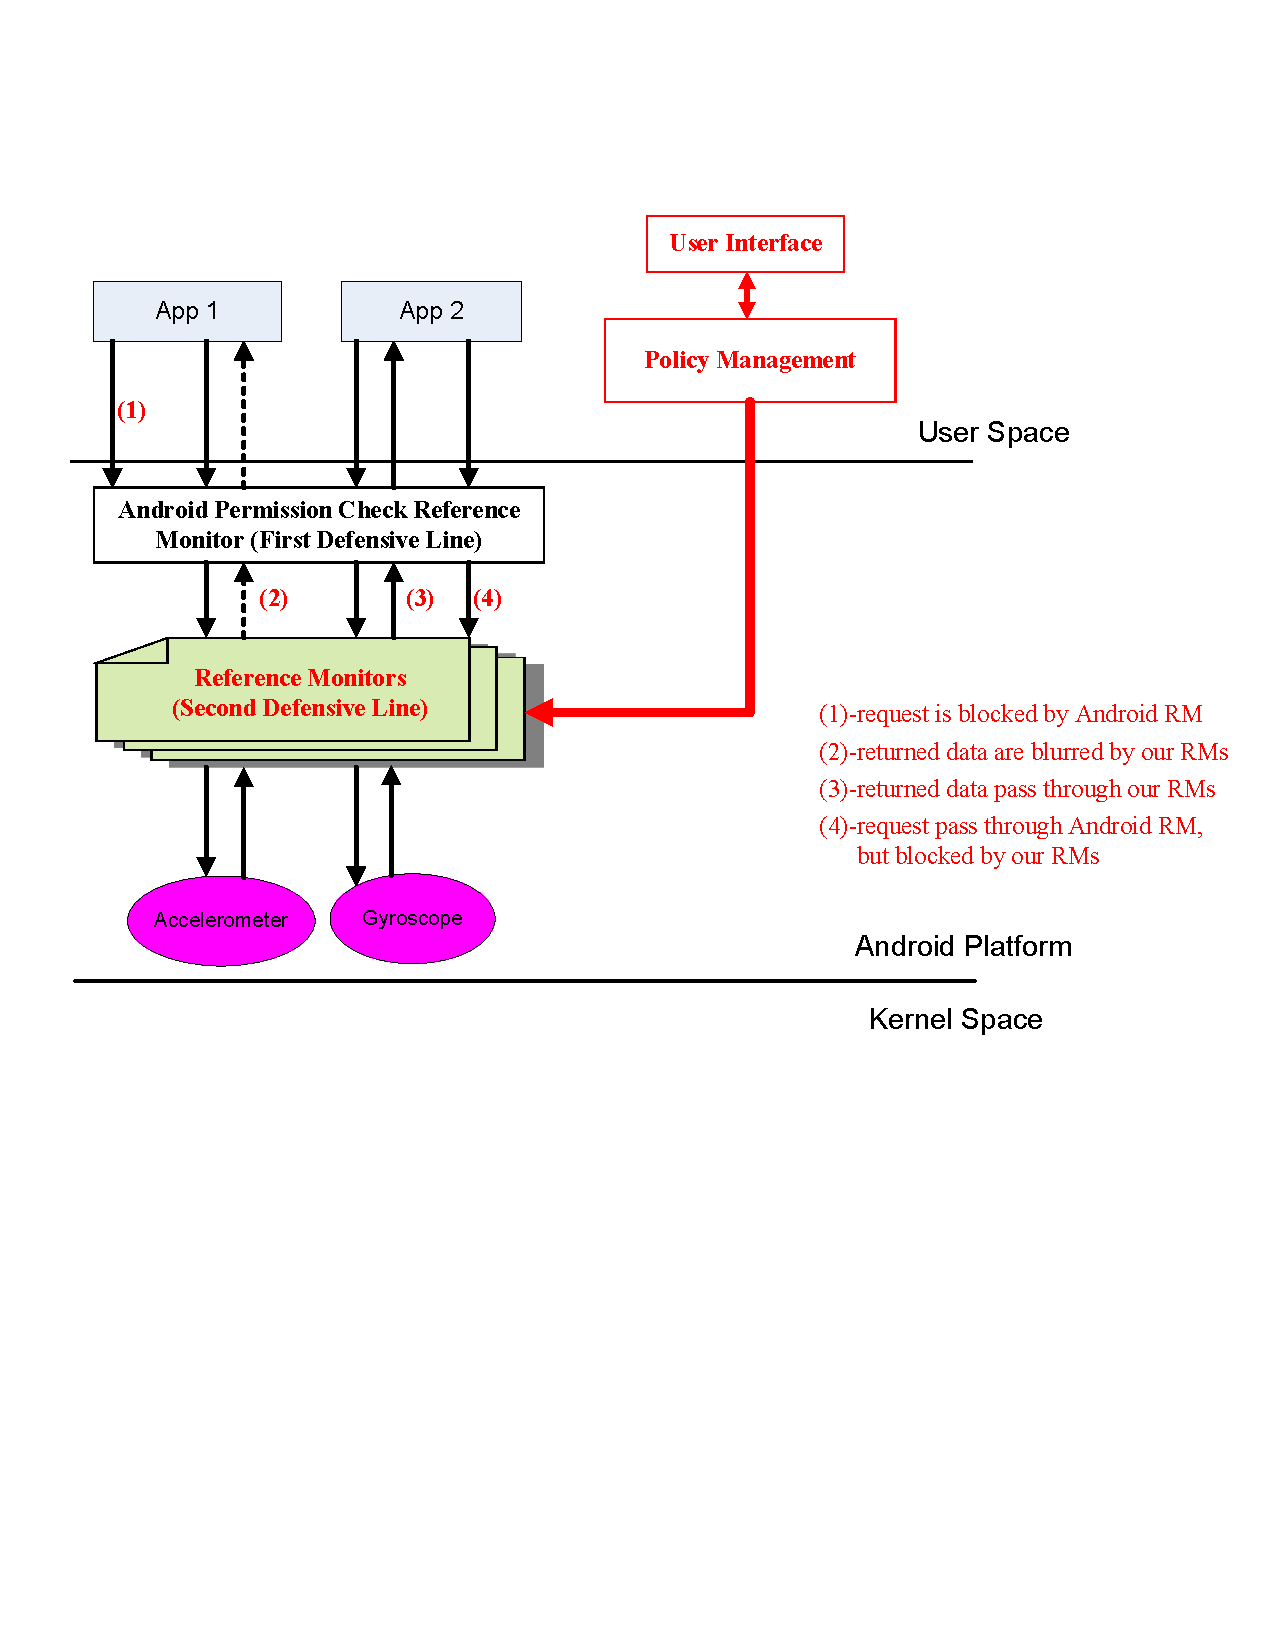
\includegraphics[width=3.7in]{refMonDesign.pdf}\\
  \caption{System architecture based on reference monitors.}
  \label{Fig:design}
\end{figure}

The BlurSense project deals with this problem of fine-grained conrol of sensor data
by requiring that all untrusted apps be installed
through an app that filters sensor data through a reference monitor~\cite{cappos2014blursense}.  
(See Figure~\ref{Fig:design})
The policy for filtering can be set by the user based on a trust metric.
 The reference
monitor can exercise fine-grained control to degrade the accuracy of the sensor data, render it 
completely meaningless, or pass it through unchanged.  
In the case of geolocation, GPS measurements can be set to the center of the nearest
large city or random noise can be added.  Another approach would be to allow the user to decide
whether to in stall the app or not, based on the trust evaluation 
%based on the sensor data requested in the manifest file.
The reference monitor approach poses less risk than others; the worst that can happen is
that the app will have the same access to the sensor data that
is permitted by the manifest file. In the best case, BlurSense
would limit the access to sensor data based on a combination of trust metrics for the app.
BlurSense is currently able to filter data on battery level, CPU usage, geolocation (latitude, longitude,
altitude, accuracy, and speed if available), and network related measurements
(mobile network type and operator, nearby WiFi access point
and Bluetooth devices).

\eat{
Currently, implemented sensor modules and
the available contextual information are classified into three
categories: device specific (percentage of battery power level,
CPU and memory utility), location related (latitude, longitude,
altitude, accuracy, and speed if available), and network related
(mobile network type and operator, nearby WiFi access point
and Bluetooth devices). While sensor modules are the system
hooks with read access to valuable sensor resources, they
cannot manipulate sensor data. Additionally, the sensor API
also provides a base registry service with a common interface
for use by a sensor implementation. } % end comment
\eat{For both local and remote
processes to access sensor data, a JSON/sl4a library
is incorporated to provide data in an unified format. In case
newer sensors appear on future mobile devices, developers can
add newly implemented sensors into this framework rather
easily. 
%The registry service listens for connection on a set of predefined ports via XML-RPC. 
Thus, both local and remote
process can connect to these ports and register for sensor
updates.
Our preliminary work in this area has resulted in working 
code~\cite{seattle-sensor-git}, tutorials~\cite{seattle-sensor-project}, and a 
blog for problem discussion~\cite{sensor}. Several different groups have
already used our early-stage proof-of-concept to solve problems across a variety
of domains, demonstrating the potential of sharing sensor data. 
} % end comment

  % description of the experiments: comparisons of driving data
\input{results}  
\section{Conclusion}
With the growing number of mobile devices owned by ordinary citizens all around the world and an increase of their participation in the network traffic generation and data provided, the problem of an evaluation of the trust, which other collaborators may have in the quality and security of their data and devices becomes more and more important. The presented trust evaluation framework includes procedures and tools to evaluate trust in mobile devices and applications, in particular in Android based smartphones. The framework hierarchical structure allows for incorporating multiple diverse factors affecting trust evaluation as well as facilitates its extension.
The current framework version includes the evaluation procedures based on the analysis of the following factors: the content of applications installed and executed, the device’s operating system settings and configuration, level of privacy supported by the devices and applications, patterns of the battery drain and CPU and network bandwidth usage. The conducted empirical study demonstrated a significant difference between the change of voltage in the cases of an execution of normal applications and the same applications with embedded additions, such as for example advertising. Another study produced distinguished patterns of the CPU and network use.
The framework includes not only the procedures of the trust evaluation but also the methods of its verification. 
Trust verification and adjustment could be performed through comparison of data received from different data sources on the 
same device as well as by comparing the data originated from various devices. The significant discourse between data 
originated from various sources should results in decreasing trust assessment for the corresponding data sources and devices. 
In the paper, we have described a comparative study of the speed measurements obtained from a car speedometer sensor and the speed calculated 
with the GPS location sensor measurements. This illustrates how the framework could be employed not only for trust evaluation 
but also for detecting various anomalies, which might include malicious attacks against the mobile devices.



% \section*{Acknowledgment}
% Weiss was supported by the National Science Foundation through grant TUES-1141341 
% Cappos was supported by the National Science Foundation through grants 

\bibliographystyle{abbrv}
\bibliography{bibdata}

\end{document}

